\section{Riflessione e rifrazione}
\subsection{Riflessione}
Per analizzare il fenomeno della riflessione abbiamo verificato la legge di Cartesio (riportata sotto), misurando gli angoli di incidenza e riflessione della microonda su uno specchio riflettente.
\begin{equation}
    \theta_i=\theta_r
\end{equation}
\noindent
Gli angoli ricavati, misurati in gradi, sono i seguenti:

\begin{table}[h!]
    \centering
    \begin{tabular}{cccc}
    $\theta_i \, (^\circ)$ && \,$\theta_r \, (^\circ)$&\\
    \toprule
    20	&20	&&21\\
    20	&21	&&23\\
    30	&31	&&31\\
    30	&29	&&27\\
    40	&37	&&35\\
    40	&35	&&39\\
    50	&43	&&48\\
    50	&44	&&43\\
    60	&65	&&69\\
    60	&63	&&63\\
    \bottomrule
    \end{tabular}
    \caption{}
    \label{}
\end{table}

Abbiamo osservato che per angoli piccoli l'errore era maggiore, supponendo che ciò fosse dovuto al fatto che emettitore e ricevitore si trovassero troppo allineati. Probabilmente il ricevitore captava il segnale non solo dell'onda riflessa ma anche di quella emessa.
\subsection{Rifrazione}
Abbiamo studiato il fenomeno della rifrazione con lo scopo di misurare l'indice di rifrazione dello styrene, un idrocarburo aromatico.
Abbiamo posizionato un contenitore di polistirolo a base triangolare sulla pedana al centro. Dopo aver verificato che l'indice di rifrazione del polistirolo fosse pari a quello dell'aria abbiamo misurato l'angolo tra l'ipotenusa e il cateto maggiore attraverso le formule trigonometriche, l'angolo risultava essere di $\theta_v = 22,54 ^\circ$.

\begin{figure}[h!]
    \centering
    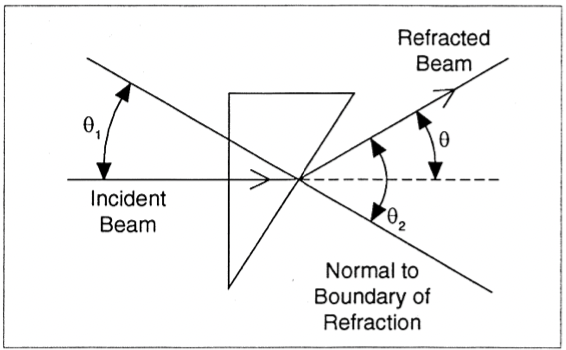
\includegraphics[scale=.7]{Immagini/triangolo.png}
    \caption{}
    \label{triangolo}
\end{figure}
 
In seguito abbiamo preso l'angolo formato con la normale, $\theta_n = 38,54 ^\circ$, da cui abbiamo ricavato il valore di n = 1,63 come indice di rifrazione dello styrene. Quest'ultimo è stato calcolato attraverso la seguente relazione:
$$
n=\dfrac{\sin\theta_n}{\sin\theta_v}
$$
